\section{Data Acquisition}
\label{sec:chap_lidar_data_acquisition}

In this section, we report on the relevant characteristics of the four sensors used in our dataset. We then describe the physical configuration of our test setup, then outline the weather condition pertaining to each of the six collected snowfalls. Finally, we describe how the information from the LiDARs was preprocessed before analysis.

\subsection{Sensors}

Data acquisition was performed with the following four LiDARs: the SICK LMS200, SICK LMS151, Hokuyo UTM-30LX-EW, and the Velodyne HDL-32E. Relevant sensor information is provided in Table~\ref{tab:lidars}, but the reader is referred to the manufacturers' documentation for additional information\footnote{Available here: Velodyne~\citep{VelodyneManual}, Hokuyo~\citep{UTMDatasheet}, LMS151~\citep{LMS151Datasheet}, LMS200~\citep{LMS200Manual}}.

The first element that gives a qualitative overview of the sensor performance is the maximum acquisition distance. This value depends on several factors, such as lighting conditions and target remission. This value is provided directly for the HDL-32E and UTM-30LX-EW, but based on a target remission greater than \SI{75}{\percent} for the LMS200 and LMS151. Another element to consider is the shape and area covered by the beam, which influences the probability of hitting a snowflake as well as the proportion of area it covers. A final significant element which changes from one sensor to the other is the number of echoes returned. The Hokuyo sensor can return up to three echoes, which means that it could locate two snowflakes before the beam reaches the ground. Regarding the LMS151, two echoes are evaluated by the hardware, but only one is returned. Finally, note that all LiDARs use class 1 laser with a wavelength of \SI{905}{\nano\meter}.

\begin{table}
    \centering
    \begin{tabular}{@{}llrrc@{}}
        \toprule
        \textbf{Sensor} & \textbf{Spot shape} & \makecell[cc]{\textbf{Spot area} \\ (at 30 meters)} & \makecell[cc]{\textbf{Maximum} \\ \textbf{distance}} & \textbf{Echoes} \\
        \hline
        SICK LMS200         & Circle    & \SI{165}{\centi\meter\squared} & \SI{28}{\meter} & 1 \\
        SICK LMS151         & Circle    & \SI{22}{\centi\meter\squared}  & \SI{50}{\meter} & 2 \\
        Hokuyo UTM-30LX-EW  & Ellipse   & \SI{196}{\centi\meter\squared} & \SI{30}{\meter} & 3 \\
        Velodyne HDL-32E    & Rectangle & \SI{51}{\centi\meter\squared}  & \SI{70}{\meter} & 1 \\
        \bottomrule
    \end{tabular}
    \caption[Overview of characteristics specific to each \gls*{lidar}.]{Overview of characteristics specific to each \gls*{lidar}.}
    \label{tab:lidars}
\end{table}

\subsection{Setup Configuration}

Data acquisition was conducted at Pouliot Hall of Laval University, where sensors were placed close to the inner wall of a window facing N\SI{50}{\degree}E. As shown in Figure~\ref{fig:setup}, a wooden structure held the sensors side by side at approximately \SI{14}{\meter} above the ground. The main scanning plane (i.e. XY plane in the sensor reference frame) formed a \SI{30}{\degree} angle with respect to the building wall, so as to increase the maximum distance as much as possible without having the laser beams hitting  trees or a pedestrian walkway present near the building. In addition, an RGB camera was placed alongside the LiDARs to provide visual information about the scene. In this configuration, a slight opening of the window allowed to keep the instruments inside while scanning outside. To avoid direct interference between sensors, corrugated plastic layers were placed between them. Figure~\ref{fig:view} shows the scene as observed by the RGB camera placed with the sensors.

\begin{figure}
    \centering
    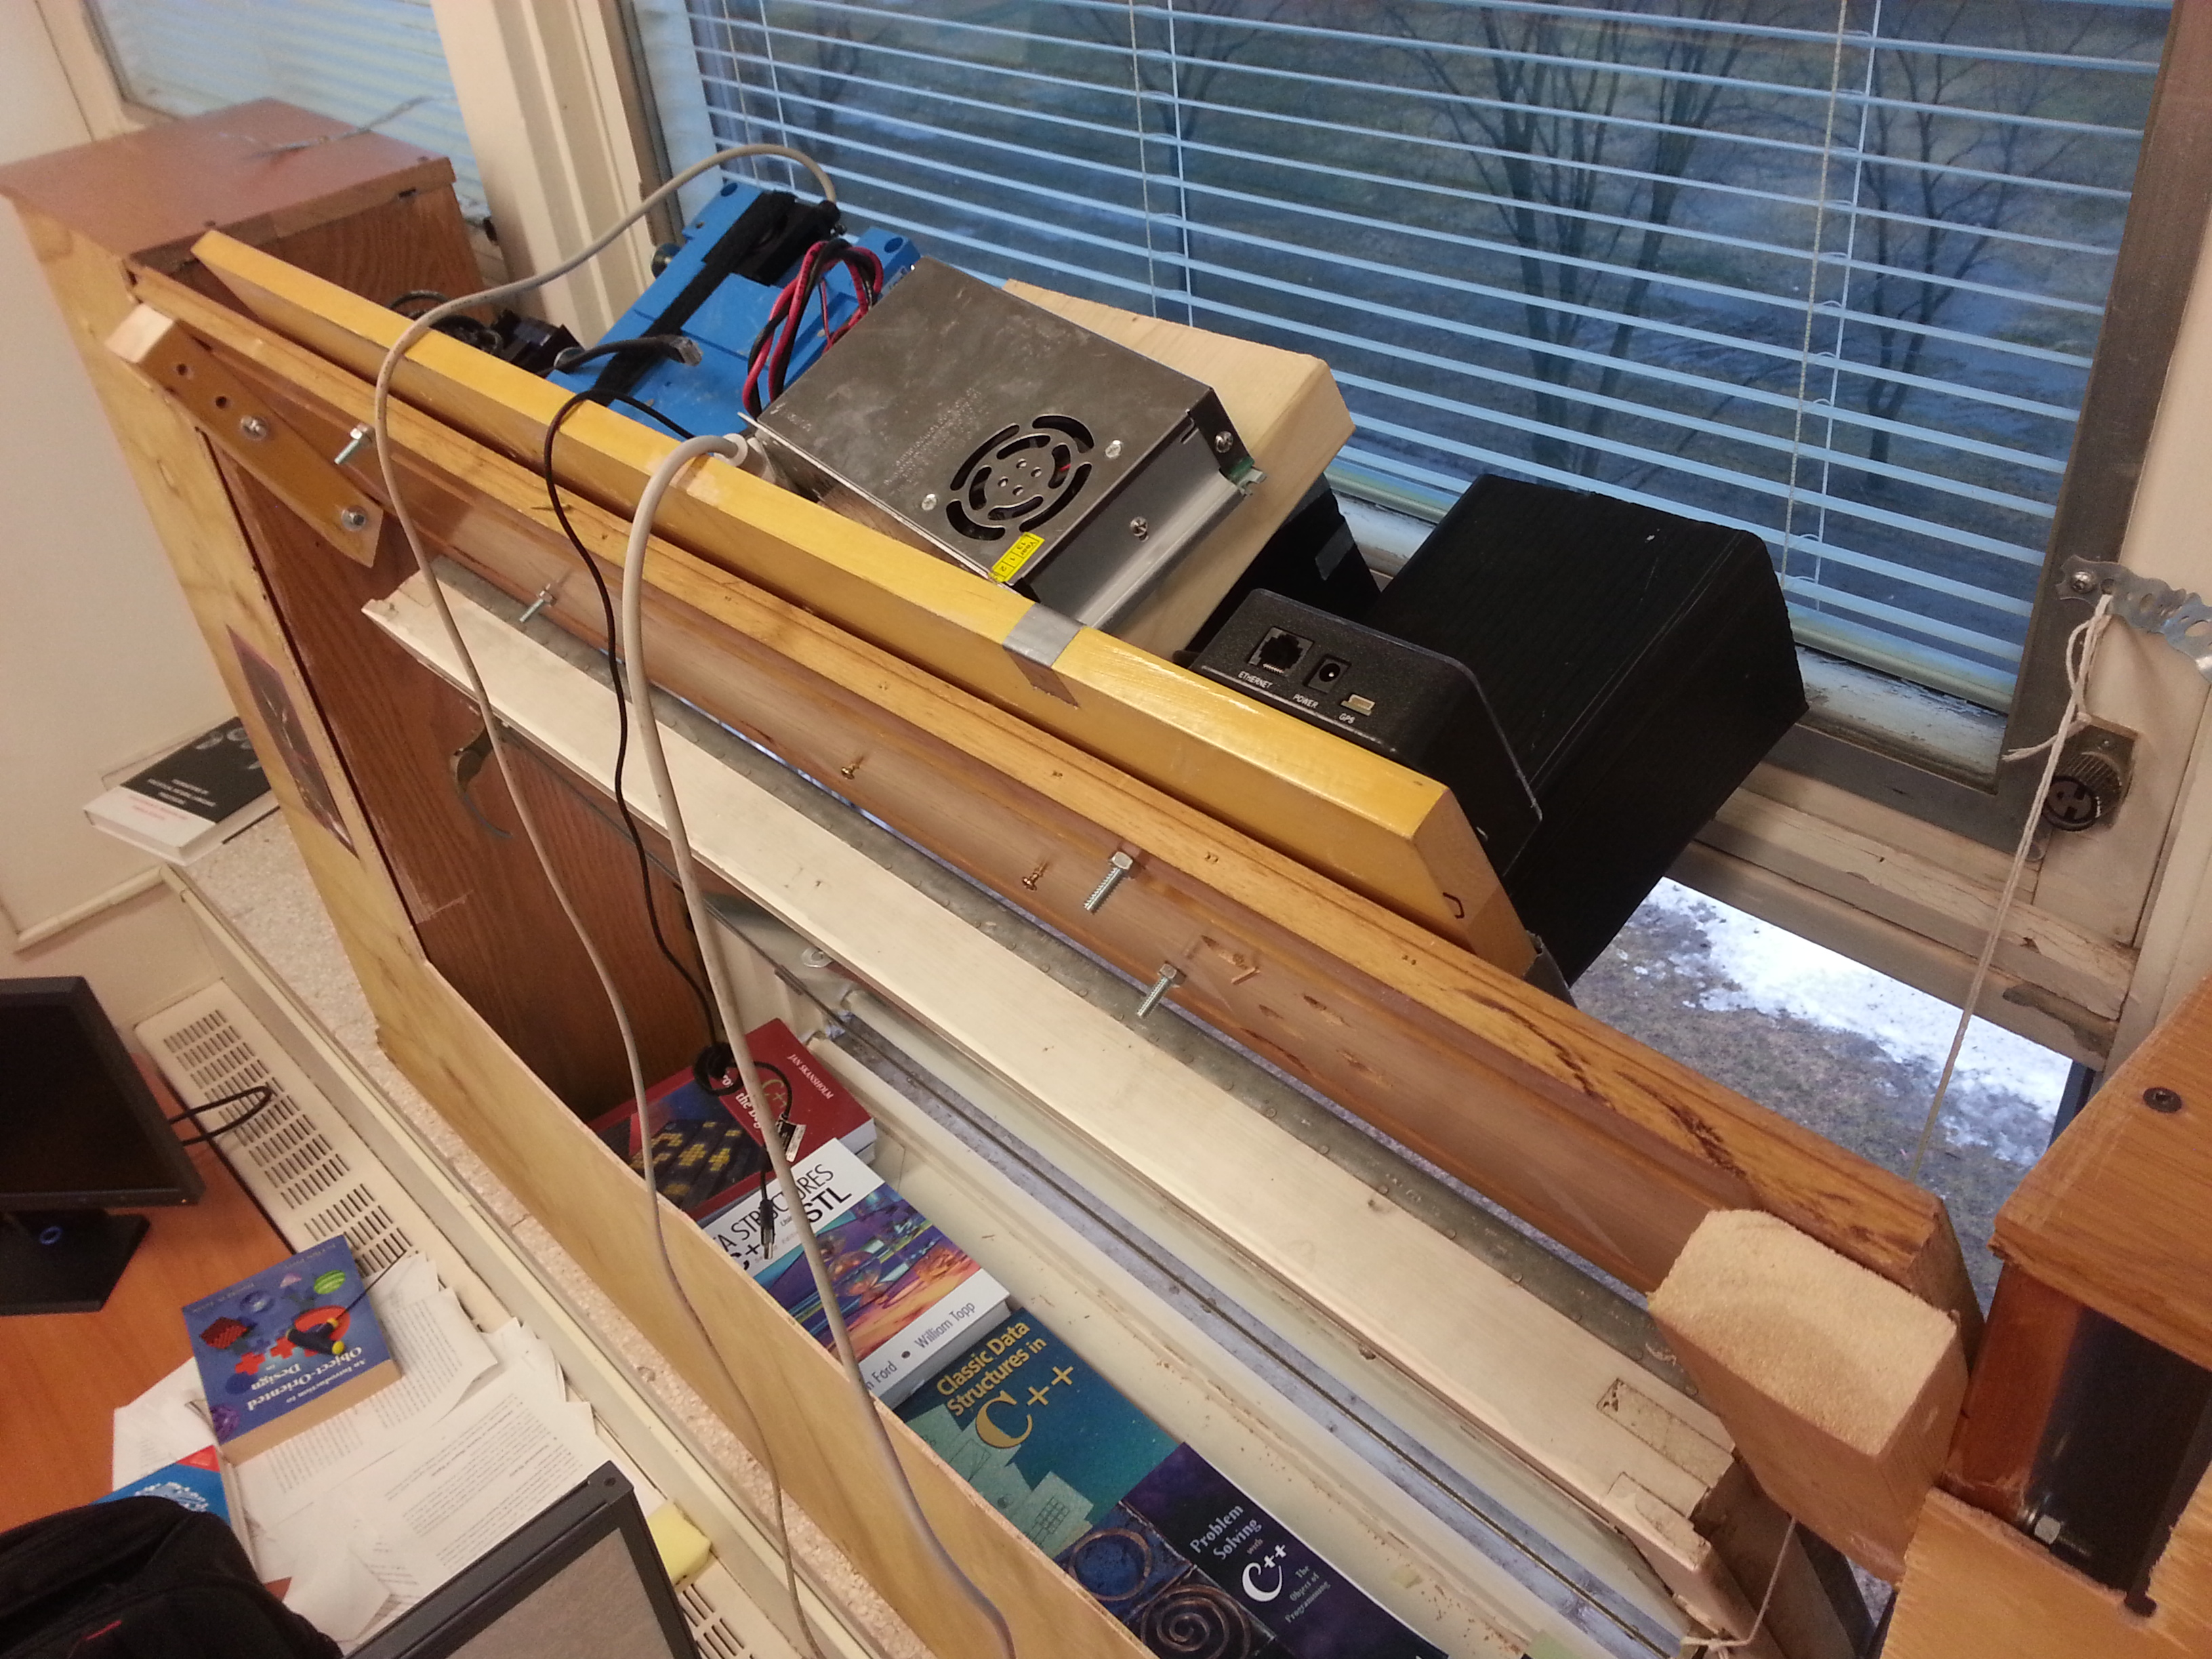
\includegraphics[width=0.80\linewidth]{./img/chap_lidar/setup_diag.png}
    \caption[The experimental setup.]{The experimental setup. The 3D axis represent the orientation of the sensors and the bottom left panel represent the 2D geometry as seen from the right side of the picture.}
    \label{fig:setup}
\end{figure}

\begin{figure}
    \centering
    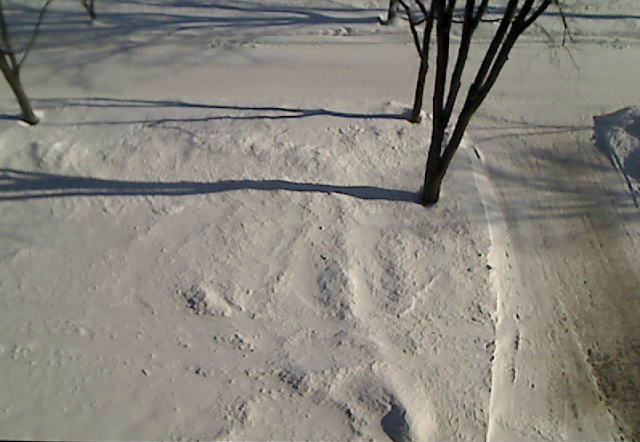
\includegraphics[width=0.80\linewidth]{./img/chap_lidar/camera_view.jpg}
    \caption[View from the camera.]{View from the RGB camera.}
    \label{fig:view}
\end{figure}

\subsection{Dataset Description}
Data acquisition started February~12 and ended on March~2. A total of 10 episodes were collected for a total of more than 50 hours of data. Recordings were made using the Robot Operating System (ROS)~\citep{ROSWeb}, which provides standardized data types as well as time synchronization. Data was acquired at different times of day and in a wide variety of conditions, covering a wide range of snowflakes size, falling rate and wind speed.  Table~\ref{tab:overview-dataset} provides an overview of our data\footnote{Wind speed, daily precipitation and temperature are reported from Québec City Jean Lesage International Airport at approximately \SI{9}{\km} from Laval University. Data is available here \citep{WeatherCanada}.}. Of these, six are used in the current study, as highlighted in this table.

\begin{table}
    \centering
    \begin{tabular}{@{}lllllrr@{}}
        \toprule
        \makecell[lc]{\textbf{Beginning} \\ \textbf{time}} & \makecell[lc]{\textbf{Duration} \\ (HH:MM)} & \makecell[lc]{\textbf{Snowflakes} \\ \textbf{size}} & \makecell[lc]{\textbf{Falling} \\ \textbf{rate}} & \makecell[lc]{\textbf{Wind speed} \\ \textbf{range} \\ (\SI{}{\km\per\hour})} & \makecell[cc]{\textbf{Daily pre-} \\ \textbf{cipitation} \\ (\SI{}{\cm})}  & \makecell[cc]{\textbf{Temperature} \\ (\SI{}{\celsius})} \\
        \hline
        \makecell[lc]{\textbf{Feb 12,} \\ \textbf{9:47 am}}  & 09:21 & Small      & Variable & [2--13]  & 1.4 & -14.1 \\
        \makecell[lc]{Feb 14, \\ 10:12 pm}                   & 04:12 & Small      & Very low & [5--13]  & 0.2 & -21.4 \\
        \makecell[lc]{\textbf{Feb 19,} \\ \textbf{8:38 am}}  & 10:02 & Big/small  & High     & [3--28]  & 4.5 & -10.9 \\
        \makecell[lc]{Mar 2, \\ 1:06 pm}                     & 01:27 & Big/small  & Variable & [22--36] & 1.6 & -9.1  \\
        \makecell[lc]{Mar 3, \\ 10:33 pm}                    & 02:17 & Big        & Medium   & [7--9]   & 5.4 & -13.3 \\
        \makecell[lc]{\textbf{Mar 4,} \\ \textbf{11:45 am}}  & 04:12 & Big/medium & Low/none & [20--30] & 2.0 & -4.3  \\
        \makecell[lc]{\textbf{Mar 17,} \\ \textbf{10:08 am}} & 06:08 & Big/medium & Low/none & [1--31]  & 2.0 & -5.8  \\
        \makecell[lc]{\textbf{Mar 21,} \\ \textbf{6:44 pm}}  & 07:42 & Medium/big & High     & [5--33]  & 8.6 & -5.1  \\
        \makecell[lc]{\textbf{Mar 30,} \\ \textbf{1:06 pm}}  & 04:45 & Medium/big & High     & [4--8]   & 8.5 & -3.0  \\
        \makecell[lc]{Apr 2, \\ 1:56 pm}                     & 01:51 & Small/rain & High     & [2--10]  & 1.2 & -8.4  \\
        \bottomrule
    \end{tabular}
    \caption[Overview of our snow dataset.]{Overview of our snow dataset. Dates in bold correspond to the six days used in the present study.}
    \label{tab:overview-dataset}
\end{table}

\subsection{Pre-Selection of Laser Data}
For each sensor, we selected a combination of angles and laser rings (for the Velodyne) or angles (for the others) that had a clear view of the snow-covered ground surface. The actual details for each sensor are given in Table~\ref{tab:selectionScans}. The range of the ground in our scans was between $x = \SI{15}{\meter}$ to $x=\SI{22}{\meter}$, depending on the angle. To simplify the analysis, we considered as a snowflake echo any measurement which had a range reading of $x<\SI{14.5}{\meter}$. As will be shown later in sec.~\ref{sec:chap_lidar_histo}, this approximation is valid as the vast majority of those events happened for $x<\SI{10}{\meter}$. %Thus, any snowflakes echoes between $x>\SI{14.5}{\meter}$ and the snow-covered ground surface were negligible, for all four sensors.

\begin{table}
    \centering
    \begin{tabular}{@{}lrllr@{}}
        \toprule
        \textbf{Sensor} & \textbf{Acquisition frequency} & \textbf{Selected beams/angles} & \textbf{Selected rings} & \textbf{Window size} \\
        \hline
        LMS200          & \SI{9.375}{\Hz}       & 55--115                & N/A               & ~\SI{106}{\second} \\
        LMS151          & \SI{25.000}{\Hz}      & 310--220               & N/A               & ~\SI{40}{\second}  \\
        Hokuyo          & \SI{20.000}{\Hz}      & 440--590               & N/A               & ~\SI{100}{\second} \\
        Velodyne        & \SI{10.000}{\Hz}      & -0.05--0.25 rad        & 17--31            & ~\SI{40}{\second}  \\
        \bottomrule
    \end{tabular}
    \caption[Details of measurement selection for the analysis.]{Details of measurement selection for the analysis. The window size is the temporal window used to calculate statistics during the temporal evolution of a snowfall.}
    \label{tab:selectionScans}
\end{table}

\FloatBarrier
